\documentclass[a4paper,11pt]{article}

\usepackage[T1]{fontenc} \usepackage{lmodern} \usepackage[utf8]{inputenc}
\usepackage[english]{babel} \usepackage{csquotes}
\usepackage{float} \usepackage{graphicx,subfigure,epstopdf}
\usepackage{amssymb,amsmath} %\usepackage{siunitx}
\usepackage[nodayofweek]{datetime}
\usepackage[top=3.5cm,bottom=2.5cm,left=3cm,right=3cm,headheight=30pt]{geometry}
\usepackage[style=numeric,backend=biber]{biblatex} \bibliography{refs}
\usepackage{fancyhdr} \pagestyle{fancy} \usepackage{lastpage}
\usepackage{parskip} \setlength{\parskip}{.5em} \setlength{\parindent}{1em}
\usepackage[colorlinks=true,allcolors=blue]{hyperref} \hypersetup{
	pdfauthor={Michaël Defferrard, Soroosh Shafiee},
	pdftitle={Incremental Gradient Methods},
	pdfsubject={Project proposal}
}
\lhead{Advanced Topics in Data Sciences\\ Project proposal}
\chead{\hspace{2cm}EPFL\\ \hspace{2cm}\shortdate\today}
\rhead{Michaël \textsc{Defferrard}\\ Soroosh \textsc{Shafiee}}
\cfoot{}

\newcommand{\R}{\mathbb{R}}
\newcommand{\B}{\mathcal{B}}
\newcommand{\eqnref}[1]{(\ref{eqn:#1})}
\newcommand{\prox}{\textrm{prox}}
%\DeclareMathOperator*{\prox}{prox}

\begin{document}

\begin{center}
	\Large{\textbf{\textsc{Incremental Gradient Methods}}}
\end{center}

This project is aimed to be a way for us to better understand and thinker with
the recent advances in the Stochastic Gradient Descent algorithms, specifically
the recent SAGA \cite{defazio_saga_2014}. This method is similar in spirit to
the previously developed SAG, SDCA, MISO and SVRG. This class of algorithms have
been developed to solve problems of the form
\begin{equation} \label{eqn:problem}
	\min_{x \in \R^d} \frac{1}{n} \sum_{i=1}^n f_i(x) + h(x),
\end{equation}
where each $f_i$ is convex and has Libschitz continuous derivatives with
constant $L$ or is strongly convex with constant $\mu$; and $h$ is a convex but
potentially non-differentiable function (his proximal operator is however easy
to compute). While computing the full gradient would be prohibitive due to large
$d$ and $n$, these iterative stochastic algorithms reduce the computational cost
of optimization by only computing the gradient of a subset of the functions
$f_i$ at each step.

Many machine learning problems can be cast in \eqnref{problem}, such as
(constrained) Least-Square or Logistic Regressions with $\ell_1$ or $\ell_2$
regularization; where $x$ would represent the model parameters, $f_i$ the data
fidelity term applied to a particular sample $i$, and $h$ a regularization or
indicator function of a convex set. As such, these methods are of use in our
respective domains of expertise: Signal Processing on Graphs and Risk Analytics.

In this project we explored two approaches to modify the SAGA algorithm:
\begin{itemize}
	\item A \textbf{memory-efficient SAGA}, by way of computing and storing
		gradients over mini-batches instead of single sample, as is done for the
		infamous Stochastic Gradient Descent. It turns out that is approach is
		also faster than the original algorithm because it exploits the
		vectorial instructions of modern processing units.
	\item A \textbf{distributed SAGA}, by way of distributing the gradient
		computation over many CPU cores while fusing the results and updating
		the model parameters on the master.
\end{itemize}

\section{SAGA algorithm}

The algorithm starts with some known initial vector $x^0 \in \R^d$ and known
derivatives $f_i' (\phi_i^0) \in \R^d$ with $\phi_i^0 = x^0$ for each $i$. These
derivatives are stored in a table data-structure of length $n$, or alternatively
a $n \times d$ matrix. It uses a step size of $\gamma$ and, given the value of
$x^k$ and of each $f_i' (\phi_i^k)$ at the end of iteration $k$, makes the
following updates for iteration $k+1$:
\begin{enumerate}
\item Pick a $j$ uniformly at random.
\item Take $\phi_j^{k+1} = x^k$, and store $f_j'(\phi_j^{k+1})$ in the table.
	All other entries in the table remain unchanged. The quantity $\phi_j^{k+1}$
	is not explicitly stored.
\item Update $x$ using $f_j'(\phi_j^{k+1})$, $f_j'(\phi_j^k)$ and the table
	average:
	\begin{equation} \label{eqn:saga}
	w^{k+1} = x^k - \gamma \left[ f_j'(\phi_j^{k+1}) - f_j'(\phi_j^k)
	+ \frac1n \sum_{i=1}^n f_i'(\phi_i^k) \right] ,
	\end{equation}
	$$x^{k+1} = \prox_\gamma^h (w^{k+1}).$$
\end{enumerate}

\section{Memory-efficient SAGA}

We first form $\frac{n}m$ mini-batches $\{\B_i\}_i^{\frac{n}m}$ of size $|\B_i|
= m$ and take gradients w.r.t. them, such that the gradient matrix is of size
$\frac{n}m \times d$ instead of $n \times d$. The updates for iteration $k+1$
then becomes:
\begin{enumerate}
\item Pick a $i$ uniformly at random in $[1, \frac{n}m]$.
\item Take $\phi_j^{k+1} = x^k \ \forall \ j \in \B_i$, and store $\frac1m
	\sum_{j\in\B_i} f_j'(\phi_j^{k+1})$ in the table.
\item Update $x$:
	\begin{equation} \label{eqn:minisaga}
	w^{k+1} = x^k - \gamma \left[ \frac1m \sum_{j\in\B_i} f_j'(\phi_j^{k+1})
	- \frac1m \sum_{j\in\B_i} f_j'(\phi_j^k)
	+ \frac1n \sum_{i=1}^m \sum_{j\in\B_i} f_j'(\phi_j^k) \right] ,
	\end{equation}
	$$x^{k+1} = \prox_\gamma^h (w^{k+1}).$$
\end{enumerate}

Note that mini-batches can either be formed during initialization and kept
intact for the whole training. They can alternatively be formed again at the end
of each training epoch. While this is much more expensive, because the gradient
matrix has to be initialized again, we found no difference in performance.

Note that mini-batches can either be formed during initialization and kept
intact for the whole training. They can alternatively be formed again at the end
of each training epoch. While this is much more expensive, because the gradient
matrix has to be initialized again, we found no difference in performance.

\subsection{Experiments}

As the authors of \cite{defazio_saga_2014}, we tested our method on the Million
Song dataset\footnote{\url{http://labrosa.ee.columbia.edu/millionsong/}}. The
problem, as stated on the UCI repository where the data was downloaded
from\footnote{\url{https://archive.ics.uci.edu/ml/datasets/YearPredictionMSD}},
is to predict the release year of a song from audio features.

\section{Distributed SAGA}

In this section, we consider two distributed SAGA methods that is based on a parallelization of SAGA. An illustration of two methods is presented in Figure~\ref{2figs-show}. In the sequel, we let $m$ be the number of machines.

\begin{figure*} [bt]
	\centering
	\subfigure[First approach]{\label{2figs-show-a} 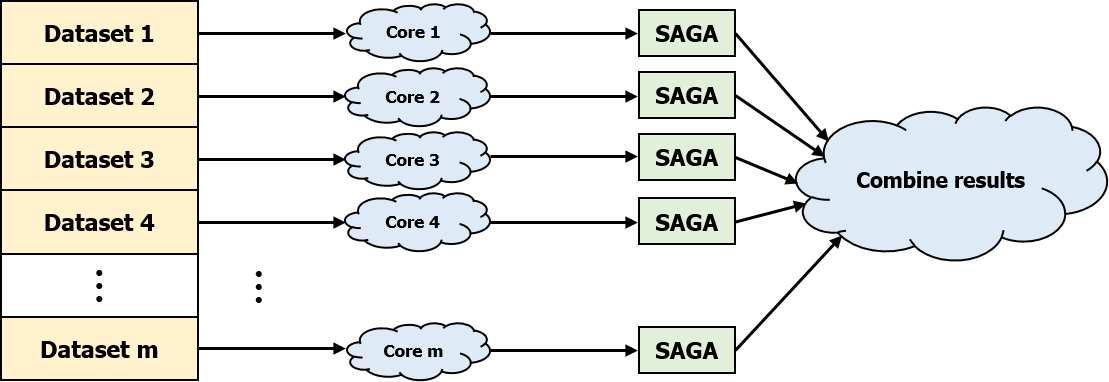
\includegraphics[width=0.48\columnwidth]{Picture2.PNG}} \hspace{0pt}
	\subfigure[Second approach]{\label{2figs-show-b} 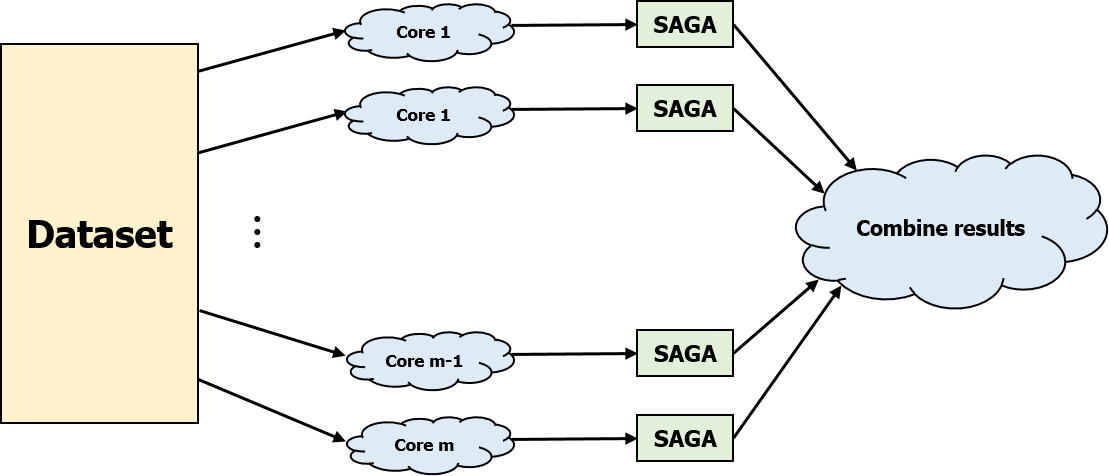
\includegraphics[width=0.48\columnwidth]{Picture1.PNG}}
	\caption{Distributed SAGA}
	\label{2figs-show}
\end{figure*}

\subsection{Distributed SAGA I}
In the first approach, we randomly partition the $n$ data points onto $m$ machines with $[n/m]$ local data points on each to parallelize the computation of \eqref{eqn:saga}. Formally speaking, at each epoch, we first partition the data to $m$ different sets. 
form $\frac{n}m$ mini-batches $\{\B_i\}_i^{\frac{n}m}$ of size $|\B_i|
= m$ and take gradients w.r.t. them, such that the gradient matrix is of size
$\frac{n}m \times d$ instead of $n \times d$. The updates for iteration $k+1$
then becomes:
\begin{enumerate}
	\item Pick a $i$ uniformly at random in $[1, \frac{n}m]$.
	\item Take $\phi_j^{k+1} = x^k \ \forall \ j \in \B_i$, and store $\frac1m
	\sum_{j\in\B_i} f_j'(\phi_j^{k+1})$ in the table.
	\item Update $x$:
	\begin{equation} \label{eqn:distsaga1}
	w^{k+1} = x^k - \gamma \left[ \frac1m \sum_{j\in\B_i} f_j'(\phi_j^{k+1})
	- \frac1m \sum_{j\in\B_i} f_j'(\phi_j^k)
	+ \frac1n \sum_{i=1}^m \sum_{j\in\B_i} f_j'(\phi_j^k) \right] ,
	\end{equation}
	$$x^{k+1} = \prox_\gamma^h (w^{k+1}).$$
\end{enumerate}

\subsection{Distributed SAGA II}

We first form $\frac{n}m$ mini-batches $\{\B_i\}_i^{\frac{n}m}$ of size $|\B_i|
= m$ and take gradients w.r.t. them, such that the gradient matrix is of size
$\frac{n}m \times d$ instead of $n \times d$. The updates for iteration $k+1$
then becomes:
\begin{enumerate}
	\item Pick a $i$ uniformly at random in $[1, \frac{n}m]$.
	\item Take $\phi_j^{k+1} = x^k \ \forall \ j \in \B_i$, and store $\frac1m
	\sum_{j\in\B_i} f_j'(\phi_j^{k+1})$ in the table.
	\item Update $x$:
	\begin{equation} \label{eqn:distsaga2}
	w^{k+1} = x^k - \gamma \left[ \frac1m \sum_{j\in\B_i} f_j'(\phi_j^{k+1})
	- \frac1m \sum_{j\in\B_i} f_j'(\phi_j^k)
	+ \frac1n \sum_{i=1}^m \sum_{j\in\B_i} f_j'(\phi_j^k) \right] ,
	\end{equation}
	$$x^{k+1} = \prox_\gamma^h (w^{k+1}).$$
\end{enumerate}

\subsection{Experiments}

\begin{figure*} [bt]
	\centering
	\subfigure[$N=10$ training samples]{\label{3figs-a} 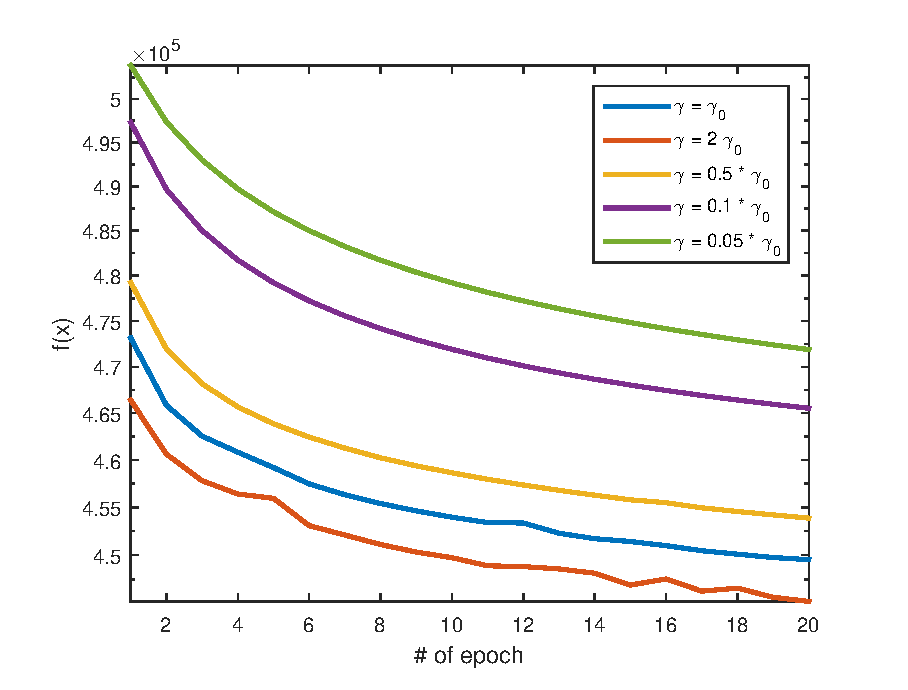
\includegraphics[width=0.31\columnwidth]{distributed1.eps}} \hspace{0pt}
	\subfigure[$N=100$ training samples]{\label{3figs-b} 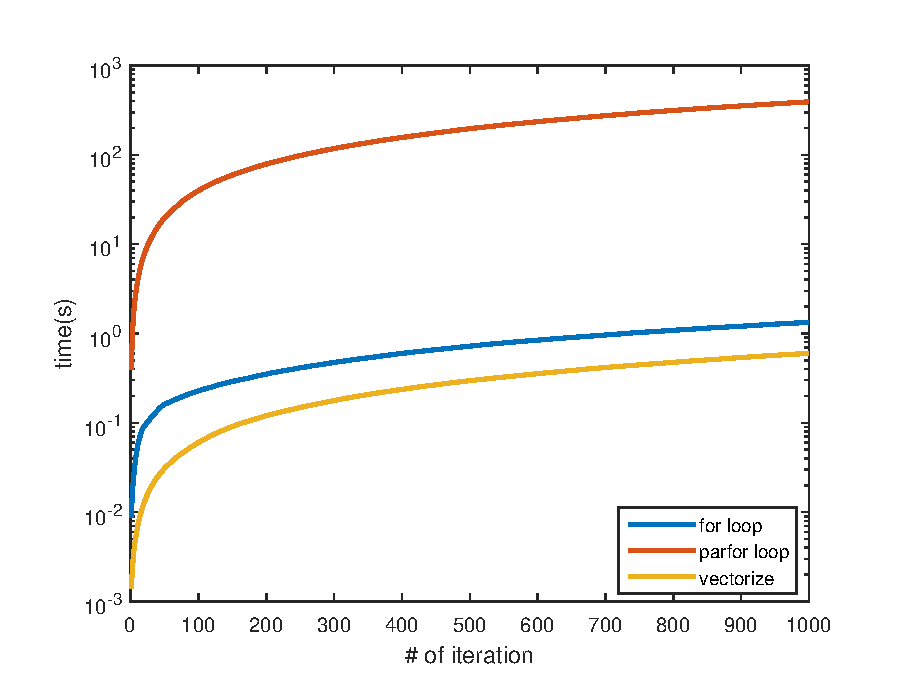
\includegraphics[width=0.31\columnwidth]{distributed2.eps}} \hspace{0pt}
	\subfigure[$N=1000$ training samples]{\label{3figs-c} 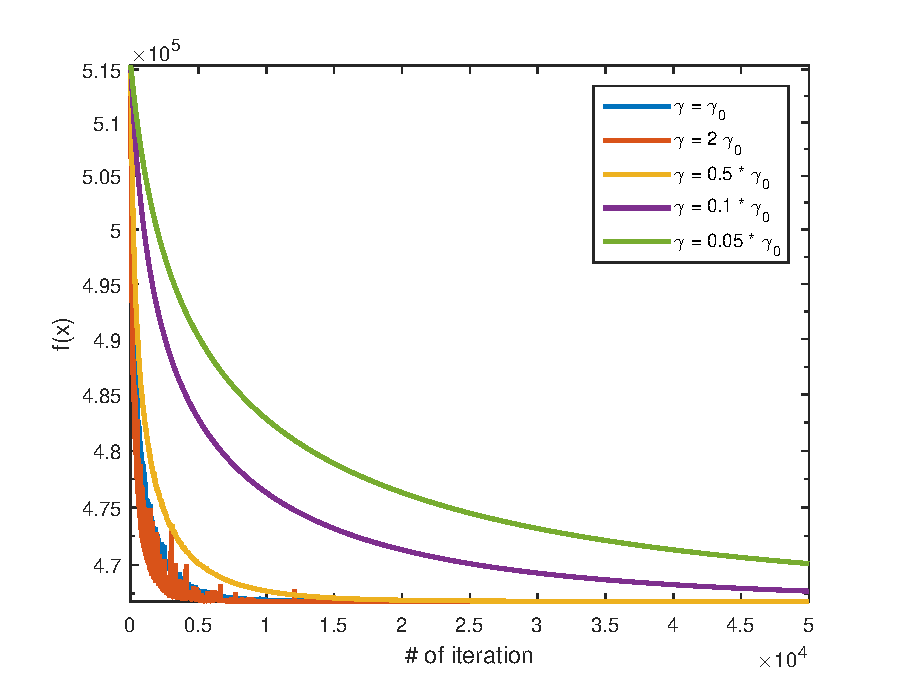
\includegraphics[width=0.31\columnwidth]{distributed3.eps}}
	\caption{Out-of-sample performance (solid blue line) and the average CCR (dashed red line)}
	\label{3figs}
\end{figure*}

\begin{figure*} [bt]
	\centering
	\subfigure[$N=10$ training samples]{\label{2figs-a} 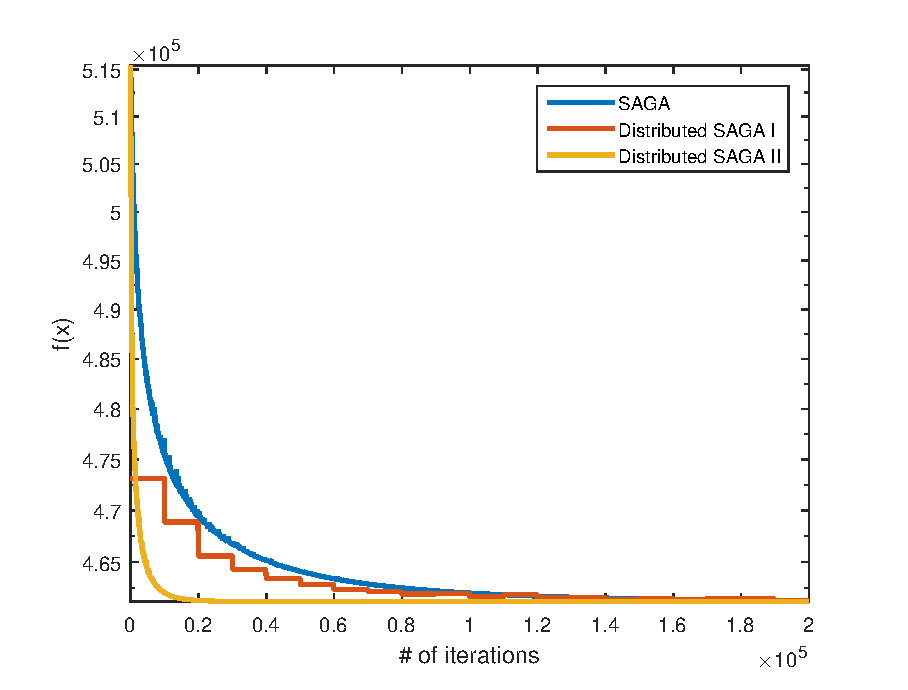
\includegraphics[width=0.48\columnwidth]{compare.eps}} \hspace{0pt}
	\subfigure[$N=100$ training samples]{\label{2figs-b} 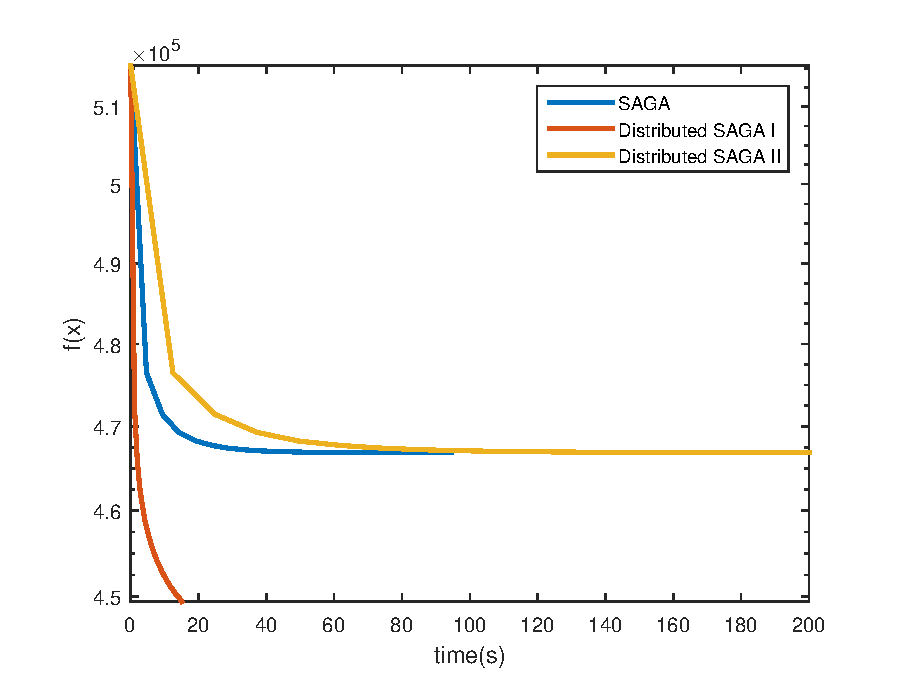
\includegraphics[width=0.48\columnwidth]{compare2.eps}}
	\caption{Out-of-sample performance (solid blue line) and the average CCR (dashed red line)}
	\label{2figs}
\end{figure*}

\printbibliography

\end{document}
